\smallframetitle

\section{From 24/06/24 to 28/06/24}
\insertsectionframe

\subsection{New ideas on neighbours detection}
\insertsubsectionframe

\begin{frame}{Neighbours detection without Delaunay}
    Just to see, we asked ourselves: why not trying to find neighbours without the Delaunay triangulation? Here is our methodology:

    \begin{block}{Creating the potential-neighbours-graph}
        The base idea was to firstly create a graph. But how?

        We will use the maximum distance to connect base stations according to the distance criteria,
        i.e. we connect a base station to surrounding stations that are in the radius of $max\_distance$.
    \end{block}

    And then we apply the angle and quadrant criteria like before.
    
    \begin{block}{Is it worth it?}
        It gives results that are more or less the same than before, but there are some imperfections.
        So, we could say that this is interesting but not really useful.
    \end{block}
\end{frame}

\subsection{Here come\dots}
\insertsubsectionframe

\begin{frame}{\dots a newer database!}
    Because the other databases we found earlier were not really convincing (in fact they are just useful to compare results).
    We therefore did some other research and found some interesting things!

    \begin{block}{ANFR}
        The National FRequency Agency, a public administrative body, was set up by the Telecommunications Regulation Act of 26 July 1996
        to plan, manage and monitor the use of public radio frequencies in France.
    \end{block}

    \begin{block}{The database itself}
        In this database\footnotemark, you have a map of all base stations in France. The interest of this database is that we can have all the frequencies used in one site and the orientation of the antennas.

        However, the problem is that we cannot download this database.
    \end{block}

    So, let's find a downloadable database.

    \footnotetext{\url{https://www.cartoradio.fr/\#/cartographie/stations}}
\end{frame}

\begin{frame}{\dots a newer database! - bis}
    This is another database from ANFR. This time we have the frequencies used in the databases.
    
    We linked those results in the first database by only keeping the highest frequency per base station.
\end{frame}

\subsection{Analysis of Frequency Data for Mobile Operators in France}
\insertsubsectionframe

\begin{frame}{France spectrum - mobile network frequency plan}
    We have detailed data on the frequency spectrums used by mobile operators in France. This data allows us to understand the specific frequencies at which each base station operates.
    \begin{block}{Frequency Bands:}
        \begin{itemize}
            \item The primary frequency bands used for 4G LTE in France include 700 MHz, 800 MHz, 1800 MHz, 2100 MHz, and 2600 MHz.
            Each frequency band has its own characteristics in terms of range, penetration, and data capacity.
        \end{itemize}
    \end{block}
    \begin{figure}
        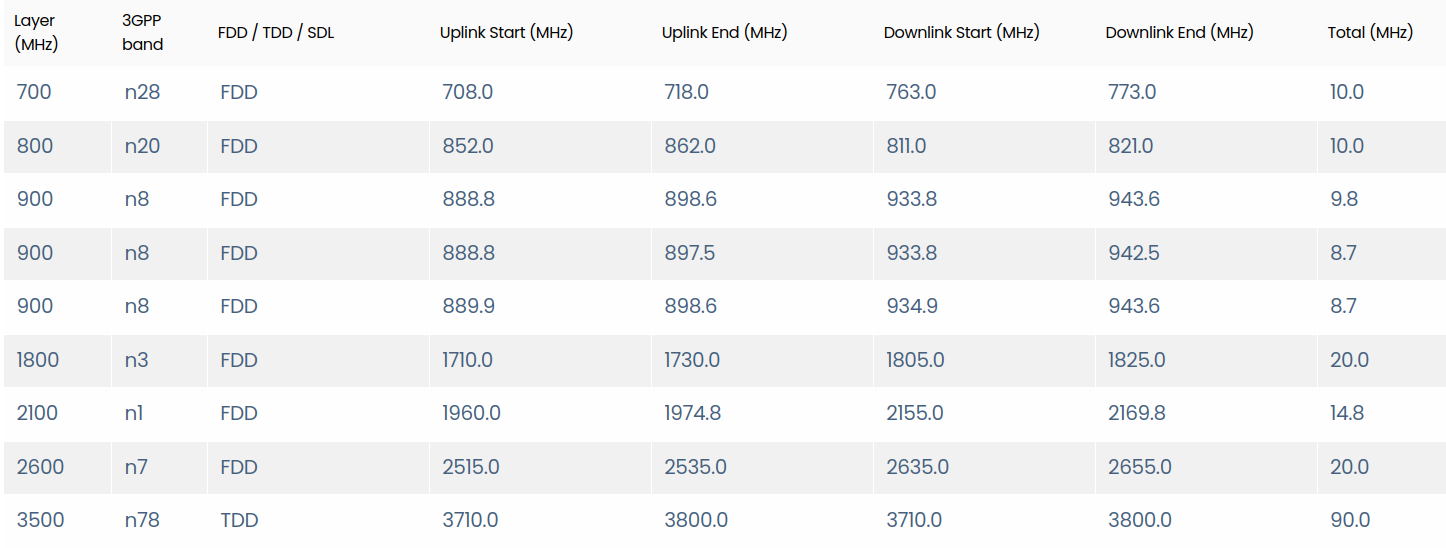
\includegraphics[height=0.4\paperheight]{images/Altair/Or_spectrum.png}
        \caption{Orange Mobile network frequency plan}
    \end{figure}
\end{frame}

\begin{frame}{Analysis of Frequency Data for Orange}
    \begin{figure}
        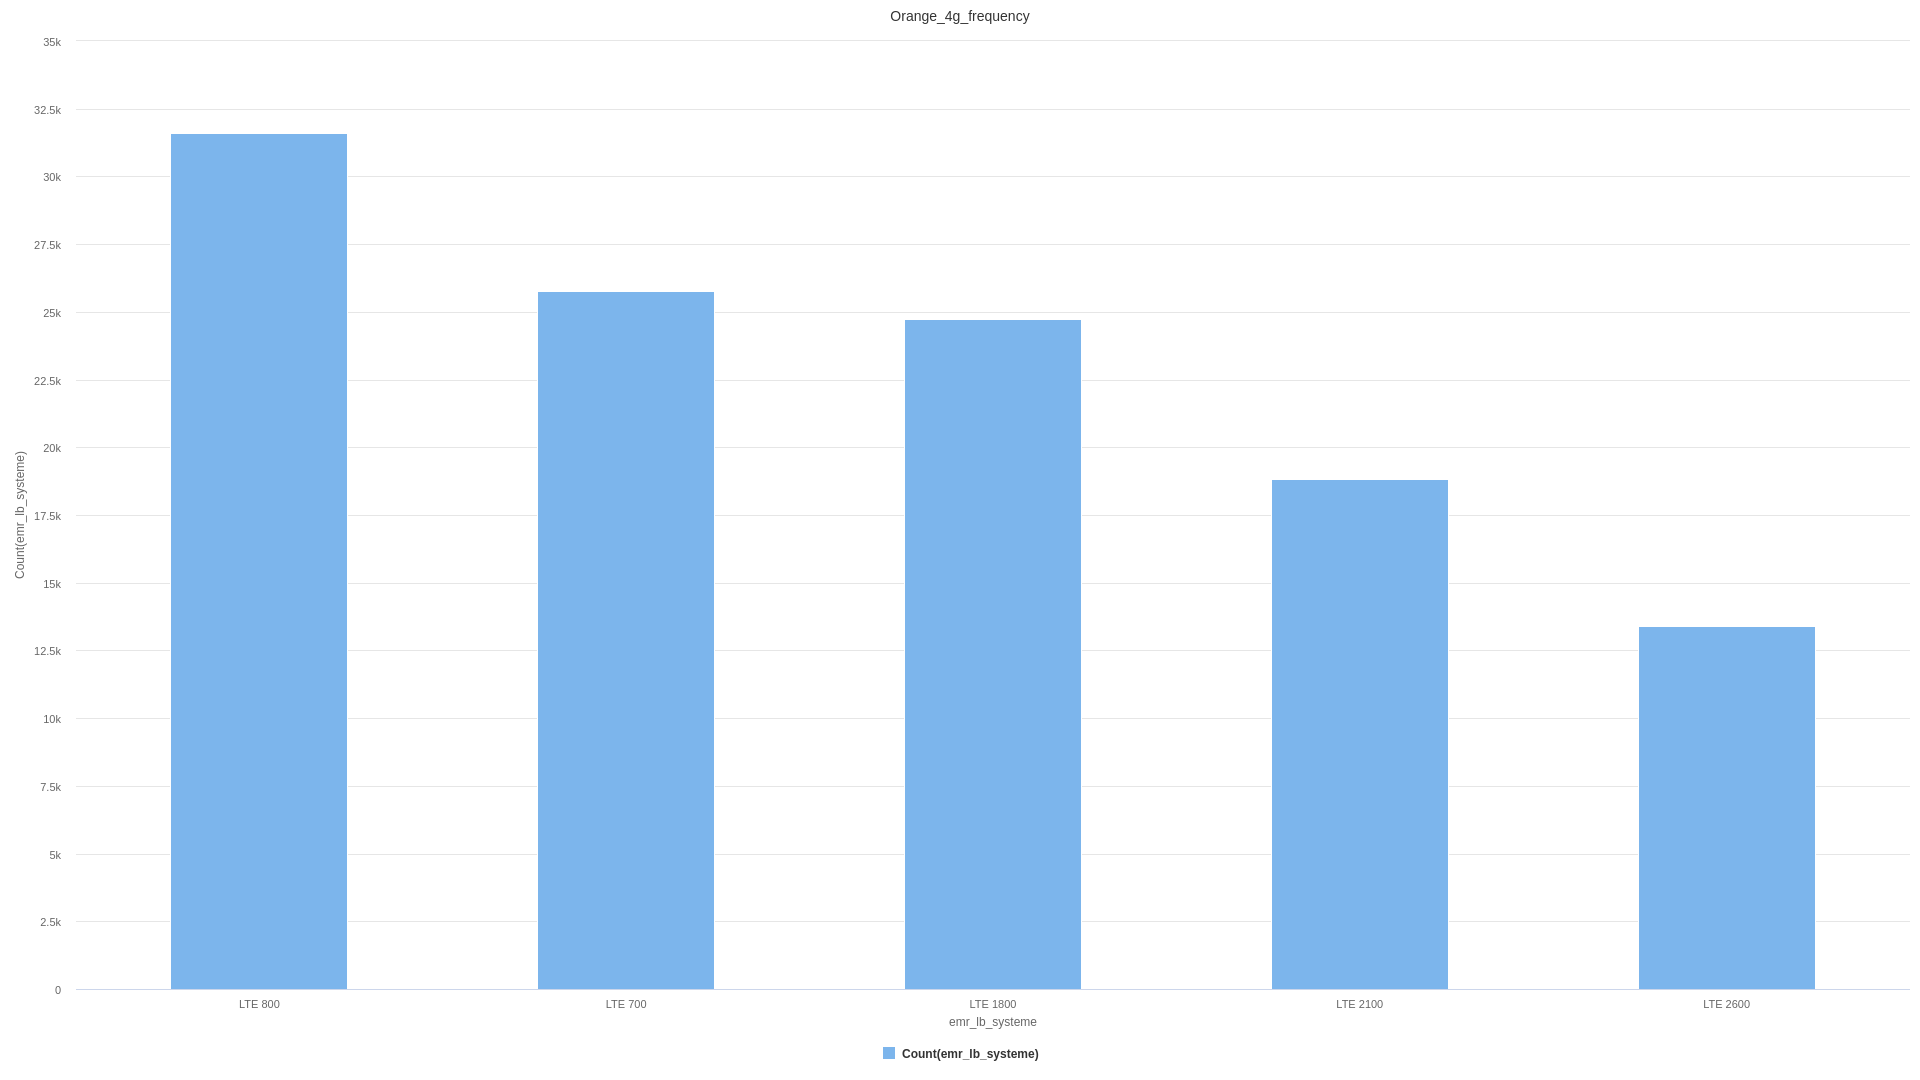
\includegraphics[height=0.6\paperheight]{images/Altair/Or_4g_freq_compar.png}
        \caption{Count of antennas operating at each frequency band}
    \end{figure}
\end{frame}

\begin{frame}{Analysis of Frequency Data}
    \begin{block}{Characteristics of each band}
        \begin{itemize}
            \item 700 MHz and 800 MHz: Long-range, good building penetration.
            \item 1800 MHz and 2100 MHz: Balanced range and capacity.
            \item 2600 MHz: Short-range, high capacity.
        \end{itemize}
    \end{block}

    \begin{block}{Methodology for Coverage Calculation}
        To estimate the coverage zones of mobile base stations using only frequency data, we can implement the following approach. 
        
        We can apply standard radio propagation models such as the Hata Model for urban areas and the Cost-231 for suburban and rural areas.
        These models allow us to estimate coverage zones based on the operating frequency of each base station. Despite lacking specific data on transmission power, antenna gain, path loss, and receiver sensitivity, these propagation models provide a generalized prediction of signal coverage areas by leveraging established empirical data and frequency characteristics.
        This methodology can enable us to approximate the coverage zones for each frequency band.
    \end{block}
\end{frame}

\begin{frame}
    \frametitle{LTE RF Link Budgeting Model}
    \begin{itemize}
        \item The link budget calculations are needed for the calculation of cellular coverage parameters.
        \item A link budget takes into consideration all the losses and gains involved in equipment (e.g., BTS), end-terminals (e.g., mobile devices), and communication medium (e.g., free space).
        \item The results obtained indicate the maximum allowable propagation loss (MAPL). The formulae used in the link budget calculations are expressed below:
    \end{itemize}
    \begin{block}{Link budget calculations}
        \begin{align}
            EIRP_{Tx} &= P_{Tx} + G_{Tx} - L_b \\
            EIRP_{Tx} &= NB_{noise} + Th_{noise} + SINR \\
            MAPL &= EIRP_{Tx} + R_{SENS} - IM - L_{cable} + G_{Rx} - M + G_{soft}
        \end{align}
    \end{block}
    \textbf{Note:} We do not have exact data for our base stations, but we can make reasonable assumptions based on industry standards.
    \end{frame}

\begin{frame}{Reference Research Findings}
    We have referenced research that provides input parameters for radio propagation models and cell-range calculation results.
    \begin{block}{Input parameters for radio propagation model}
        \begin{itemize}
            \item Carrier Frequencys (MHz): 700, 800, 1800, and 2100 MHz.
            \item Base Station Height (hb): Typically around 30 meters.
            \item Mobile Station Height (hm): Generally around 1.5 meters.
        \end{itemize}
    \end{block}
    \begin{figure}
        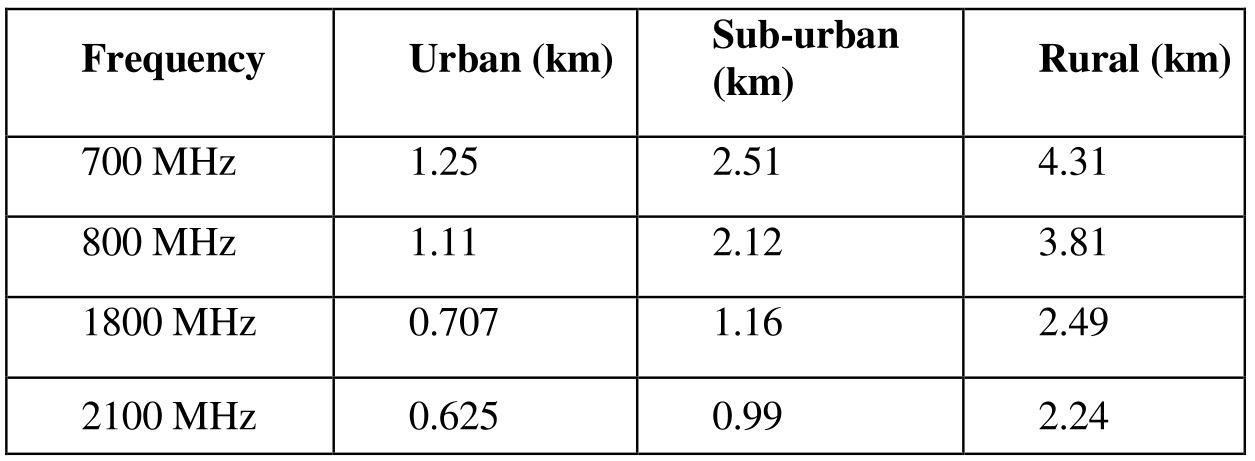
\includegraphics[height=0.35\paperheight]{images/Altair/cell_range_calc_res.png}
        \caption{Cell-range calculation results}
    \end{figure}
\end{frame}

\begin{frame}{Frequency Reuse Mode Challenges}
    \begin{columns}
        \begin{column}{0.55\textwidth}
            \begin{block}{Challenges with Unknown Frequency Reuse Mode}
                    \begin{itemize}
                        \item Each cell in a mobile network can be divided into sectors, each served by a different frequency.
                        \item The reuse of frequencies in different cells is essential to maximize the efficient use of the available spectrum.
                        \item Frequency reuse mode determines how frequencies are allocated across cells and sectors to minimize interference.
                        \item We lack detailed information on the specific frequency reuse mode utilized for each sector of our base stations.
                        \item Assumptions about uniform frequency reuse may not reflect the actual, varied configurations used in practice.
                    \end{itemize}
            \end{block}
        \end{column}
        \begin{column}{0.6\textwidth}
            \begin{figure}
                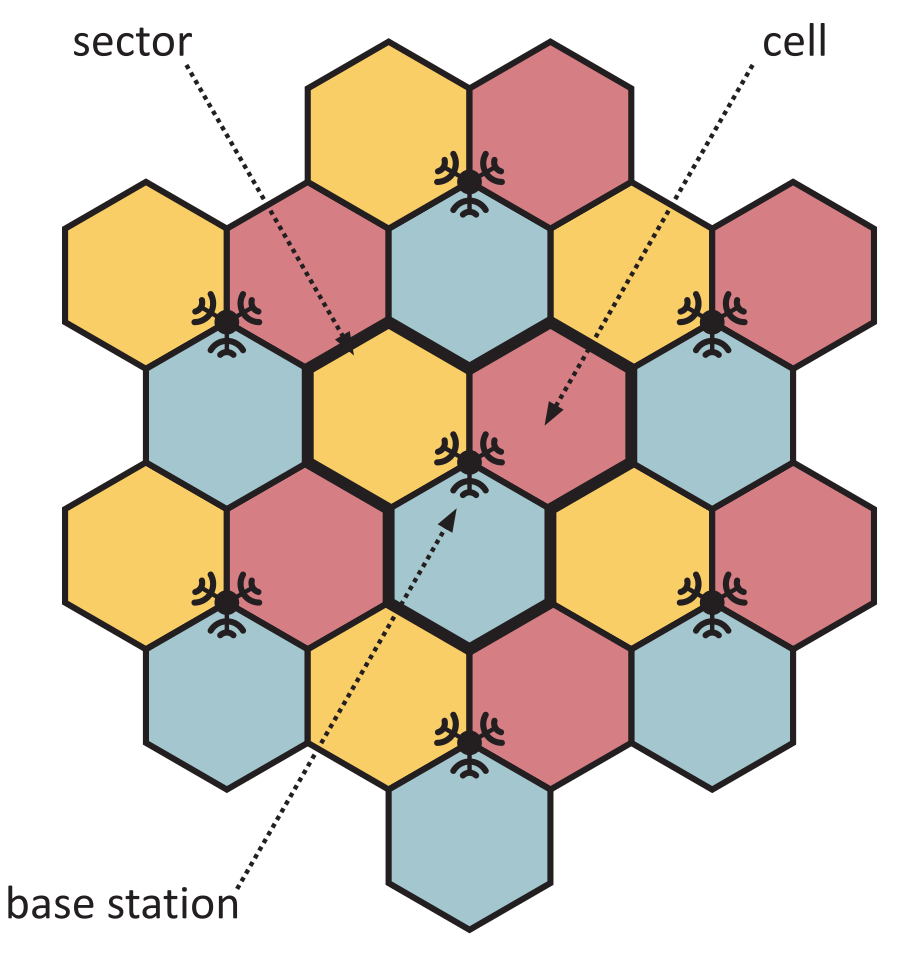
\includegraphics[height=0.4\paperheight]{images/Altair/Sectorization.png}
                \caption{Sectorization}
            \end{figure}
        \end{column}
    \end{columns}
\end{frame}